\section{Введение}
\label{sec:Chapter1} \index{Chapter1}
Аргументационная теория, или аргументация, является междисциплинарным исследованием о том, как выводы могут быть достигнуты через череду логических рассуждений. Извлечение аргументации – область науки, стоящая на стыке обработки естественного языка, информационного поиска и непосредственно аргументационной теории.

В общем виде аргумент состоит из утверждения и набора предпосылок, связанных с этим утверждением. Утверждение и предпосылки называются компонентами аргументации. Связи между ними могут выражать не только структуру аргумента, но и тип отношения внутри нее – поддержку или опровержение. Данные отношения называются полемической позицией аргументации.
\begin{figure}[H]
 \setcounter{figure}{0}
 \captionsetup{justification=raggedright,singlelinecheck=false,labelfont=bf,labelsep=period,name={Рисунок}}
 \centering{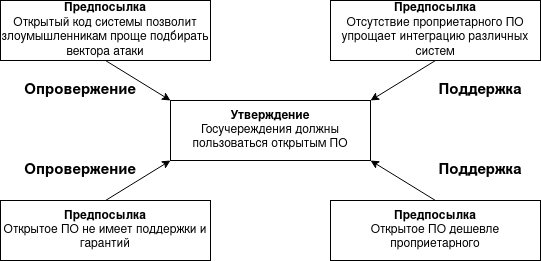
\includegraphics[scale=0.65]{Аргумент.png}}
 \caption{Пример аргументов, относящихся к применению открытого ПО.}
\end{figure}

%Помимо вышеуказанных структурных особенностей связи компонент аргументации могут дополнительно описываться следующими характеристиками:
%\begin{itemize}
%    \item Сила – мера того, насколько предпосылки соглашаются с утверждением, темой или опровергают их.
%    \item Общность – мера того, насколько утверждение или предпосылка раскрывает тему, а не ее конкретные примеры, иначе оно превращается в факт.
%    \item Авторитетность - характеристика того, насколько данное утверждение или предпосылка обоснована. Например высказывание ученого о глобальном потепленее авторитетнее высказывания политика.
%\end{itemize}

Аргументация присутствует почти во всех источниках информации: она встречается в бытовых спорах, дебатах, научном дискурсе. Особый вид политической аргументации – пропаганда является ключевым компонентом некоторых интернет-ресурсов.

За последнее десятилетие сильно вырос интерес к автоматическому выделению аргументации \cite{lippi2016argumentation}. Этому поспособствовал прорыв в области обработки естественного языка, заключающийся создании предобученных нейросетевых моделей с сильными обобщающими способностями \cite{mikolov2013efficient, devlin2018bert, radford2019language}. Несмотря на то, что данные модели содержат в себе знание общеизвестных и часто встречаемых фактов, выученных из больших коллекций \cite{petroni2019language}, они не способны применять узкоспециализированую информацию. Для решения данного недостатка используют графы знаний и другие онтологии \cite{sorokin2018modeling, chen2019multi}, однако их создание требует трудоемкий и долгий процесс ручной разметки данных экспертами. Автоматическое извлечение аргументации позволяет динамически извлекать специализированную информацию и структурировать ее.

В данной задаче отстутствует устоявшаяся постановка. В научной литературе существует несколько вариантов определения аргументации и соответстующих подходв к ее выделению. Из-за этого отсутствует общепринятый набор тестов и метрик, позволяющих оценить качество системы извлечения аргументации. Следствием отсутствия универсальной постановки задачи является небольшое число исследовательских групп, занимающихся аргументацией, наличие различных по постановке и небольших по размерам обучающих коллекций и почти полное отсутствие развития задачи на языках отличных от английского.

Проблему плохого покрытия языка можно решать созданием новых или параллельных \cite{fishcheva2019cross}  корпусов, а также методикой межязыкового переноса знаний \cite{ponti2020xcopa, eriguchi2018zero}. Данный подход заключается в обучении мультиязычной модели на одном языке для адаптации полученных знаний на других языкак.

В данной работе описывается исследование методов извлечения структуры и полемической позиции аргументации, а также способы адаптации данных методов для применения на русскоязычных корпусах с помощью подхода межязыкового переноса.

\subsection{Актуальность задачи}
Извлечение аргументации можно применить во многих прикладных сценариях:
\begin{itemize}
    \item Аргументация может быть задействована в экспертных системах для получения доводов "за"  и "против" относительно какого-либо утверждения.
    \item Аргументы можно использовать в голосовых помошниках и других системах, использующих базы знаний.
    \item Выделение аргументации применительно к научным текстам позволит лучше высторить структуру взаимосвязи между цитируемыми работами.
    \item Аргументация также может использоваться для оценки убедительности и логичности текстов.
    \item Аргументация может использоваться в нефактоидных вопросно-ответных системах для ответов на вопросы, требующие объяснений: "Почему было принято следующе решение?"
\end{itemize}

Один из самых показательных примеров применения аргументации является проект IBM Debater, который способен поддерживать сложный диалог с оппонентом для обоснования определенной точки зрения. В 2019 году система IBM Debater участвовала в споре с финалистом мирового чемпионата по дебатам Харишем Натараджаном, в котором на протяжении 15 минут смогла отстаивать свою точку зрения. Другим примером могут послужить голосовые помошники, получившие широкое распространение в последние годы. В лидирующих системах, таких как Siri, Алиса, Маруся, Alexa и Google Assistant для ответов на вопросы ищутся релевантные документы, которые потом цитируются в качестве ответа, однако они не способны агрегировать информацию из нескольких источников. Добавление аргументации поможет голосовым помошникам систематизировать информацию и обосновывать свои ответы. В качестве примера можно привести работу \cite{schiller2020aspect}, где по извлеченным примерам аргументации генерируется текст.

Из всего вышесказанного можно сделать вывод, что выделение аргументации с помощью методов глубокого обучения является перспективной и актуальной задачей. Научная ценность данной работы заключается в исследовании и систематизации текущих подходов к задаче извлечения аргументации, применении новых моделей и предоставлении замеров результатов их работы. Отдельной проблемой является и работа с множеством небольших, разнящихся в постановке задачи корпусов. Следствием является и проблема построения системы извлечения аргументации для русского языка. 

В работе приводится обзор и анализ существующих работ по извлечению аргументации, предлагаются новые подходы, основанные на переносе знаний (transfer learning), а также исследуется возможность межязыкового переноса знаний для получения модели, работающей на русском языке. Дополнительно проводится интерпретация работы модели: исследуется зависимость полученных результатов в зависимости от структурных особенностей компонент аргументации, таких как наличие отрицаний, сильно окрашенных слов или антонимии.
